%manuel 6e, chapitre G3
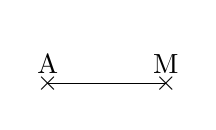
\begin{tikzpicture}[scale=1,every node/.style={scale=1}]

\draw (0,0) node [above]{A};
\draw (0,0) node {$\times$};
\draw (1.5,0) node [above]{M};
\draw (1.5,0) node {$\times$};
\draw (0,0)--(1.5,0);

\draw (0,0.7); %pour donner un peu plus de hauteur à l'image
\end{tikzpicture} 
